% uklad dokumentu
	\documentclass{article}
	\usepackage{xparse}
	\usepackage[margin=1cm]{geometry}
    \usepackage{enumerate} 
	\frenchspacing
    \linespread{1.2}
    \setlength{\parindent}{0pt}

% jezyk polski
	\usepackage[polish]{babel}
	\usepackage[utf8]{inputenc}
	\usepackage{polski}
 
% pakiety matematyczne
    \let\lll\undefined
	\usepackage{amssymb}
    \usepackage{amsthm}
	\usepackage{amsmath}
	\usepackage{amsfonts}
	\usepackage{tikz}

% hiperlacza
	\usepackage{hyperref}
	\hypersetup{
		colorlinks,
		citecolor=black,
		filecolor=black,
		linkcolor=black,
		urlcolor=black
	}

% wstawianie zdjec
	\usepackage{graphicx} 
	\pagenumbering{gobble}
	

% podstawowe informacje
    \title{Algorytmy i struktury danych - Lista 4}
    \author{P. Cegieła, W. Sęk}

\begin{document} 

\maketitle

\section{Teoretyczna złożoność}
Teoretyczne złożoności algorytmów ($n=|V|$):
\begin{itemize}
\item $k$-random - $k$ losowań ze złożonością $O(1)$ i liczenie wartości ścieżki z $O(n)$, czyli $O(kn)$,
\item $ext-neighbours$ - $n$-krotne przejście po każdym wierzchołku i przejrzenie $\frac{n(n-1)}{2}$ wierzchołków oraz policzenie wartości ścieżki z $O(n)$ daje $O(n^3)$,
\item $2-opt$ - niech $O(m)$ to złożoność przybliżenia początkowego, $l$ to liczba kroków po której się zatrzymujemy, liczenie kosztu elementu z otoczenia to $O(1)$ (przy początkowym stworzeniu tablicy pomocniczej z $O(n)$), otoczenie ma $O(n^2)$ elementów, więc całościowo $O(m+ln^2)$, gdzie $l$ zależy od przybliżenia początkowego.
\end{itemize}
\newpage
\section{Algorytm k-random}
\subsection{Tabela}
\begin{center}
\begin{tabular}{|c|c|c|c|}
\hline
\multicolumn{4}{|c|}{\textbf{Average PRD}}\\
\hline
\textbf{n} & 10-Random & 100-Random & 1000-Random\\
\hline
100 & 6413.9156401721075 & 6007.918586928952 & 5711.806977951733\\
\hline
200 & 5988.615372379403 & 5727.247304868426 & 5522.69171607988\\
\hline
300 & 5888.036831784668 & 5683.792028830031 & 5528.337270981829\\
\hline
400 & 5802.963142088209 & 5631.843379656301 & 5508.994282851\\
\hline
500 & 5779.552537965469 & 5633.505579085746 & 5517.331574583659\\
\hline
600 & 5724.137341197624 & 5578.206097637371 & 5485.583014224162\\
\hline
700 & 5711.069467439124 & 5571.201094319976 & 5476.566562989776\\
\hline
800 & 5677.560472641102 & 5562.185079759854 & 5470.719995332991\\
\hline
900 & 5673.623396583947 & 5548.007479574144 & 5481.1123195262335\\
\hline
1000 & 5650.144622314967 & 5556.232385763668 & 5459.875331845722\\
\hline
\end{tabular}
\end{center}

\subsection{Wykresy}
\begin{center}
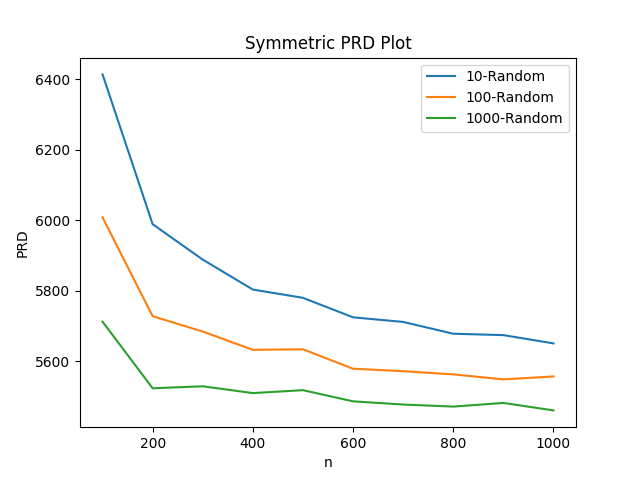
\includegraphics[width=\textwidth, 
                   height = 0.4\textheight, 
                   keepaspectratio]
                  {sym_k_random} 
\end{center}
\begin{center}
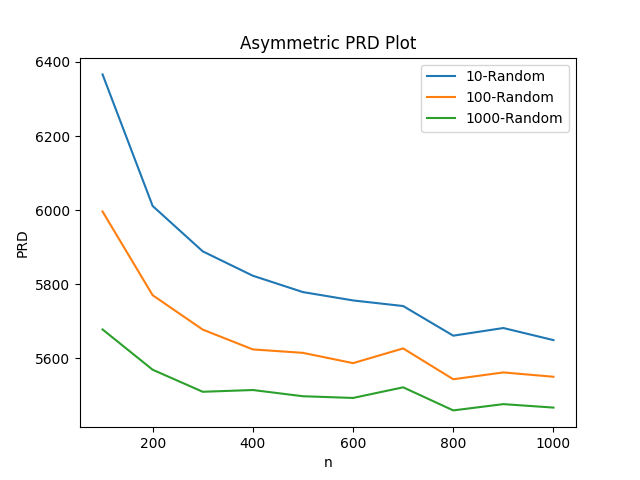
\includegraphics[width=\textwidth, 
                   height = 0.4\textheight, 
                   keepaspectratio]
                  {asym_k_random} 
\end{center}

\begin{center}
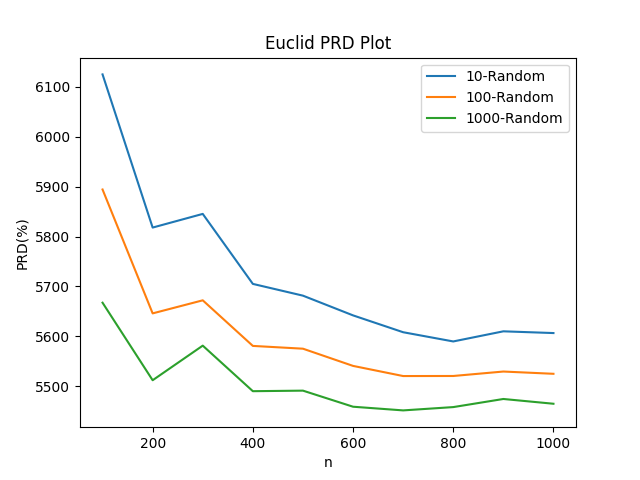
\includegraphics[width=\textwidth, 
                   height = 0.4\textheight, 
                   keepaspectratio]
                  {euc_k_random} 
\end{center}

\subsection{Wnioski}
W każdej rodzinie grafów PRD jest najmniejsze dla $k=1000$ i największe dla $k=10$, ale przy 100-krotnie większym $k$ spadek $PRD$ jest bardzo niewielki. Algorytm $k$-random radzi sobie najlepiej w rodzinie grafów euklidesowych. 

\newpage
\section{Porównanie algorytmów na grafach euklidesowych z TSPLIB}
\subsection{Tabele}
\begin{center}
\begin{tabular}{|c|c|c|c|}
\hline
\multicolumn{4}{|c|}{\textbf{Average PRD}}\\
\hline
\textbf{n} & 1000-Random & Extended-Neighbours & 2-OPT\\
\hline
51 & 306.808 & 103.146 & 91.878\\
\hline
52 & 315.237 & 98.473 & 92.241\\
\hline
70 & 435.881 & 107.926 & 97.704\\
\hline
76 & 444.027 & 111.045 & 94.849\\
\hline
100 & 593.155 & 109.201 & 95.515\\
\hline
105 & 718.542 & 107.776 & 95.285\\
\hline
130 & 656.490 & 105.463 & 93.669\\
\hline
150 & 724.239 & 100.510 & 91.808\\
\hline
225 & 964.538 & 110.576 & 94.255\\
\hline
280 & 1187.883 & 105.355 & 94.110\\
\hline
442 & 1413.942 & 106.094 & 94.210\\
\hline
1002 & 2370.379 & 111.116 & 95.631\\
\hline
\end{tabular}
\end{center}

\begin{center}
\begin{tabular}{|c|c|c|c|}
\hline
\multicolumn{4}{|c|}{\textbf{Average Time}}\\
\hline
\textbf{n} & 1000-Random & Extended-Neighbours & 2-OPT\\
\hline
51 & 31668820 & 4584170 & 8925660\\
\hline
52 & 30858480 & 5042590 & 8846290\\
\hline
70 & 42590610 & 12177150 & 27821070\\
\hline
76 & 47052070 & 15702170 & 34685250\\
\hline
100 & 61385100 & 32708000 & 87529310\\
\hline
105 & 61872570 & 42850460 & 84559130\\
\hline
130 & 74745720 & 67923570 & 131929210\\
\hline
150 & 89032240 & 103249420 & 193264830\\
\hline
225 & 134753750 & 353453680 & 717721220\\
\hline
280 & 166413550 & 664151260 & 1206655960\\
\hline
442 & 271874520 & 2618137660 & 4950646800\\
\hline
1002 & 647387380 & 30213916160 & 72123247190\\
\hline
\end{tabular}
\end{center}

\begin{center}
\begin{tabular}{|c|c|c|c|}
\hline
\multicolumn{4}{|c|}{\textbf{Maximal Time}}\\
\hline
\textbf{n} & 1000-Random & Extended-Neighbours & 2-OPT\\
\hline
51 & 39978600 & 4817900 & 9403300\\
\hline
52 & 31274700 & 5187200 & 9092600\\
\hline
70 & 47594200 & 15057800 & 32388000\\
\hline
76 & 51512200 & 19477600 & 35764400\\
\hline
100 & 65431100 & 34488100 & 96291400\\
\hline
105 & 65726300 & 62679800 & 96151900\\
\hline
130 & 79283500 & 70726100 & 136319200\\
\hline
150 & 91679000 & 105833600 & 197271000\\
\hline
225 & 162636700 & 365920200 & 774637800\\
\hline
280 & 175009000 & 688092700 & 1237435800\\
\hline
442 & 278658100 & 2660588200 & 4975043000\\
\hline
1002 & 806163300 & 30848429200 & 74493868500\\
\hline
\end{tabular}
\end{center}


\subsection{Wykresy}
\begin{center}
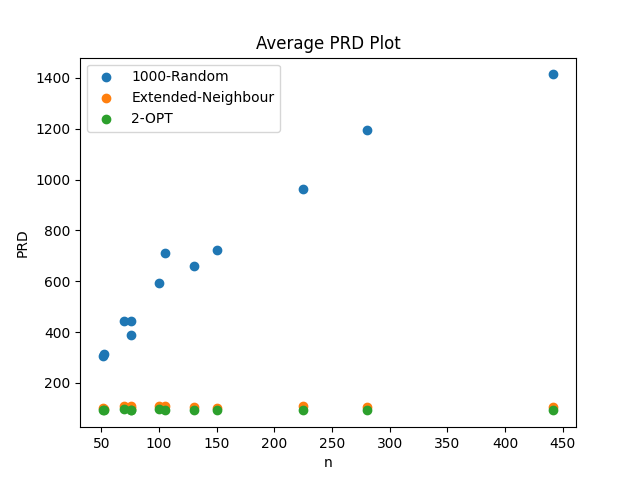
\includegraphics[width=\textwidth, 
                   height = 0.4\textheight, 
                   keepaspectratio]
                  {tsp_lib_prd} 
\end{center}
\begin{center}
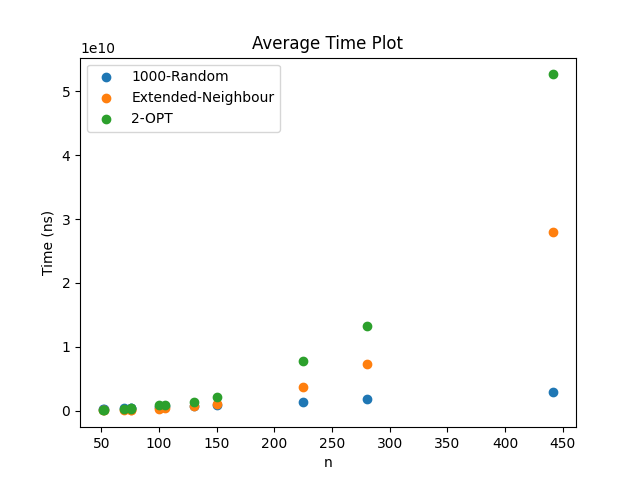
\includegraphics[width=\textwidth, 
                   height = 0.4\textheight, 
                   keepaspectratio]
                  {tsp_lib_avg_time} 
\end{center}

\begin{center}
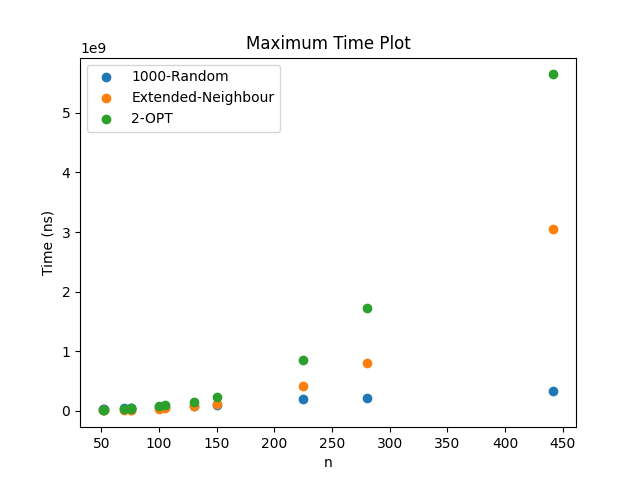
\includegraphics[width=\textwidth, 
                   height = 0.4\textheight, 
                   keepaspectratio]
                  {tsp_lib_max_time} 
\end{center}

\subsection{Wnioski}
W każdej rodzinie grafów PRD jest najmniejsze dla algorytmu $2-OPT$ i największe dla $1000-Random$, natomiast zarówno średnia i jak i maksymalna złożoność czasowa jest największa dla $2-OPT$ i najmniejsza dla $1000-Random$. Złożoność czasowa algorytmu $k$-random jest liniowa, $extended-neighbours$ jest $O(n^3)$, a $2-OPT$ ponad $O(n^3)$, ale niemożliwa do wyznaczenia ze względu na nieznaną liczbę kroków.


\section{Porównanie algorytmów na grafach generowanych losowo}
\subsection{Tabele}

\subsubsection{Grafy asymetryczne}

\begin{center}
\begin{tabular}{|c|c|c|c|c|}
\hline
\multicolumn{5}{|c|}{\textbf{Average Time}}\\
\hline
\textbf{n} & 1000-Random & Neighbours & Extended-Neighbours & 2-OPT\\
\hline
100 & 52155833 & 28571666 & 2786506666 & 30018883\\
\hline
200 & 103859000 & 1028433 & 208721416 & 214607866\\
\hline
300 & 155757366 & 2306600 & 694677850 & 716872283\\
\hline
400 & 207251383 & 4004600 & 1613402066 & 1643566000\\
\hline
500 & 256814366 & 6307966 & 3123820900 & 3195922633\\
\hline
600 & 318474116 & 8931383 & 5392548116 & 5462892666\\
\hline
700 & 373475666 & 12168183 & 8526353716 & 8648573866\\
\hline
800 & 430858466 & 15891016 & 12767540566 & 12850175766\\
\hline
900 & 485178033 & 20179966 & 18079604083 & 18253936000\\
\hline
1000 & 533764550 & 24581550 & 24880770016 & 25276480533\\
\hline
\end{tabular}
\end{center}

\begin{center}
\begin{tabular}{|c|c|c|c|c|}
\hline
\multicolumn{5}{|c|}{\textbf{Maximum Time}}\\
\hline
\textbf{n} & 1000-Random & Neighbours & Extended-Neighbours & 2-OPT\\
\hline
100 & 53740500 & 296200 & 28250900 & 31605000\\
\hline
200 & 110770900 & 1068300 & 222382100 & 217436400\\
\hline
300 & 156366900 & 2430200 & 699352300 & 730365300\\
\hline
400 & 218396100 & 4173300 & 1630130200 & 1658699700\\
\hline
500 & 272075700 & 6445900 & 3154009300 & 3248476300\\
\hline
600 & 326146900 & 9109900 & 5445648700 & 5518205200\\
\hline
700 & 392337400 & 12303600 & 8644185800 & 8705532900\\
\hline
800 & 442730100 & 16022200 & 12919136400 & 12989845300\\
\hline
900 & 497044800 & 20912700 & 18259475600 & 18320587400\\
\hline
1000 & 545819300 & 25097700 & 25367610900 & 26443099700\\
\hline
\end{tabular}
\end{center}

\begin{center}
\begin{tabular}{|c|c|c|c|c|}
\hline
\multicolumn{5}{|c|}{\textbf{Average PRD}}\\
\hline
\textbf{n} & 1000-Random & Neighbours & Extended-Neighbours & 2-OPT\\
\hline
100 & 1443.48040576265 & 53.792664503988 & 0.19841269841269842 & 0\\
\hline
200 & 2644.58297728904 & 52.564744303786 & 0 & 0\\
\hline
300 & 3443.7648431962 & 50.76765521116 & 0.9936766034327009 & 0\\
\hline
400 & 4542.2612852427 & 50.999051480909 & 0 & 0\\
\hline
500 & 5420.8049036451 & 35.213599432774 & 1.0310202617894926 & 0\\
\hline
600 & 6992.4253613068 & 49.616806843915 & 0 & 0\\
\hline
700 & 7557.8205443585 & 40.52732594919 & 0 & 0\\
\hline
800 & 8085.5198217536 & 40.938451458384 & 0 & 0\\
\hline
900 & 9265.7954870298 & 47.48286220438 & 0 & 0\\
\hline
1000 & 10006.9406083454 & 36.7679495233406 & 0 & 0\\
\hline
\end{tabular}
\end{center}


\subsubsection{Grafy symetryczne}

\begin{center}
\begin{tabular}{|c|c|c|c|c|}
\hline
\multicolumn{5}{|c|}{\textbf{Average Time}}\\
\hline
\textbf{n} & 1000-Random & Neighbours & Extended-Neighbours & 2-OPT\\
\hline
100 & 51188720 & 27634000 & 27612600 & 47058720\\
\hline
200 & 104264540 & 1104190 & 209489800 & 334344360\\
\hline
300 & 155045840 & 2350280 & 696058890 & 1092122420\\
\hline
400 & 206874620 & 4056240 & 1621604000 & 2461149340\\
\hline
500 & 252385990 & 6267200 & 3155729150 & 4642101830\\
\hline
600 & 335657920 & 9084870 & 5524767490 & 7936048030\\
\hline
700 & 404018770 & 13042890 & 8917785830 & 12985594760\\
\hline
800 & 447226030 & 16646500 & 12918400900 & 18488390450\\
\hline
900 & 489239050 & 20283590 & 18346056500 & 26428388750\\
\hline
1000 & 536137160 & 25434610 & 25319510570 & 34978626900\\
\hline
\end{tabular}
\end{center}


\begin{center}
\begin{tabular}{|c|c|c|c|c|}
\hline
\multicolumn{5}{|c|}{\textbf{Maximum Time}}\\
\hline
100 & 53478300 & 287700 & 28774700 & 59023500\\
\hline
200 & 118932100 & 1496800 & 225860300 & 374150100\\
\hline
300 & 158825400 & 2666500 & 713698900 & 1210248700\\
\hline
400 & 214809200 & 4154100 & 1651365900 & 2783661100\\
\hline
500 & 259651300 & 6437400 & 3196615100 & 4989667500\\
\hline
600 & 369051000 & 9376100 & 5731537000 & 8662696500\\
\hline
700 & 453044000 & 15011700 & 9255213200 & 14112162500\\
\hline
800 & 519034200 & 18486000 & 13176742300 & 20361935900\\
\hline
900 & 542197200 & 21026000 & 18626545300 & 27632920000\\
\hline
1000 & 587381000 & 28130500 & 26359530800 & 38144374100\\
\hline
\end{tabular}
\end{center}

\begin{center}
\begin{tabular}{|c|c|c|c|c|}
\hline
\multicolumn{5}{|c|}{\textbf{Average PRD}}\\
\hline
\textbf{n} & 1000-Random & Neighbours & Extended-Neighbours & 2-OPT\\
\hline
100 & 1696.5152490044 & 86.420983070748 & 29.828178233857 & 0\\
\hline
200 & 3364.148021938 & 86.594682621479 & 37.5914230406697 & 0\\
\hline
300 & 4675.6707100455 & 96.03524228703 & 39.851600018442 & 0\\
\hline
400 & 6264.037540901 & 92.735074436148 & 43.368040212525 & 0\\
\hline
500 & 7620.9959416362 & 94.651021903159 & 36.834144036091 & 0\\
\hline
600 & 9070.4576801556 & 105.279122298864 & 38.5508009869172 & 0\\
\hline
700 & 9992.050859801 & 105.632970306257 & 44.698984443974 & 0\\
\hline
800 & 11773.205236822 & 109.69827564215 & 43.395735797874 & 0\\
\hline
900 & 13120.7423081866 & 98.799687300712 & 43.352415182208 & 0\\
\hline
1000 & 14453.3876189813 & 96.3501317382 & 45.947937370816 & 0\\
\hline
\end{tabular}
\end{center}


\subsubsection{Grafy euklidesowe}

\begin{center}
\begin{tabular}{|c|c|c|c|c|}
\hline
\multicolumn{5}{|c|}{\textbf{Average Time}}\\
\hline
\textbf{n} & 1000-Random & Neighbours & Extended-Neighbours & 2-OPT\\
\hline
100 & 54302316 & 299333 & 29097183 & 56103983\\
\hline
200 & 110339583 & 1086783 & 222883583 & 478415716\\
\hline
300 & 157083366 & 2389250 & 718151466 & 1491255016\\
\hline
400 & 219697750 & 4206800 & 1685675166 & 3400633383\\
\hline
500 & 263064933 & 6449066 & 3270837766 & 6890312166\\
\hline
600 & 334924666 & 9413250 & 5681706716 & 12247986383\\
\hline
700 & 400039466 & 12808966 & 9070972733 & 19022276166\\
\hline
800 & 463682816 & 17058816 & 13520103633 & 29148414200\\
\hline
900 & 498106700 & 21151700 & 18577267283 & 39706015766\\
\hline
1000 & 534977600 & 25475033 & 25488625933 & 55681052150\\
\hline
\end{tabular}
\end{center}


\begin{center}
\begin{tabular}{|c|c|c|c|c|}
\hline
\multicolumn{5}{|c|}{\textbf{Maximum Time}}\\
\hline
100 & 56904000 & 321200 & 30141400 & 66528500\\
\hline
200 & 113894700 & 1158400 & 234500000 & 519662900\\
\hline
300 & 164992700 & 2442400 & 726804400 & 1549853100\\
\hline
400 & 232275800 & 4327000 & 1701320800 & 3590054900\\
\hline
500 & 286456400 & 6665100 & 3415103000 & 7359945700\\
\hline
600 & 349887600 & 9601400 & 5758347300 & 13165101000\\
\hline
700 & 426304400 & 13348700 & 9258026500 & 20301730000\\
\hline
800 & 485403100 & 18255900 & 13873937600 & 31742944800\\
\hline
900 & 510576800 & 21615300 & 18716893000 & 41209877500\\
\hline
1000 & 555995400 & 26168200 & 25734825600 & 57516775300\\
\hline
\end{tabular}
\end{center}


\begin{center}
\begin{tabular}{|c|c|c|c|c|}
\hline
\multicolumn{5}{|c|}{\textbf{Average PRD}}\\
\hline
\textbf{n} & 1000-Random & Neighbours & Extended-Neighbours & 2-OPT\\
\hline
100 & 450.17215979038 & 25.834778478913 & 11.047375520498 & 0\\
\hline
200 & 750.50161461842 & 20.382965833475 & 11.787169849889 & 0\\
\hline
300 & 955.47736955529 & 20.941890785232 & 13.4679540953857 & 0\\
\hline
400 & 1153.31540464885 & 19.2643602499013 & 11.3148715360107 & 0\\
\hline
500 & 1299.40868945165 & 19.510105455013 & 14.3355018206873 & 0\\
\hline
600 & 1471.99203529008 & 18.0634799785885 & 13.9108020407148 & 0\\
\hline
700 & 1583.07578069592 & 17.3974674441433 & 13.865053976823 & 0\\
\hline
800 & 1733.5990915691 & 20.4858325151736 & 14.038050374855 & 0\\
\hline
900 & 1844.2199324318 & 18.5850439135654 & 13.825159240164 & 0\\
\hline
1000 & 1973.2850131005 & 20.702637095026 & 14.7361632179882 & 0\\
\hline
\end{tabular}
\end{center}


\subsection{Wykresy}

\subsubsection{Grafy asymetryczne}

\begin{center}
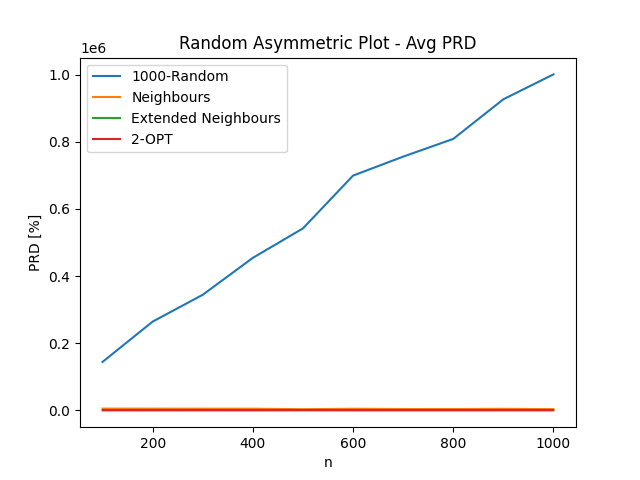
\includegraphics[width=\textwidth, 
                   height = 0.4\textheight, 
                   keepaspectratio]
                  {generated_asym_avg_prd} 
\end{center}

\begin{center}
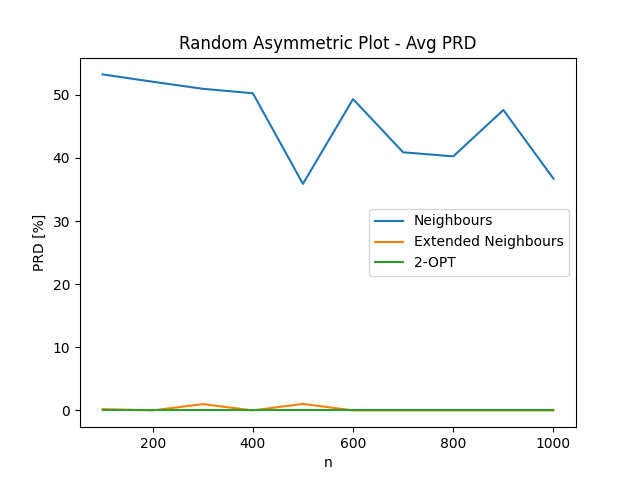
\includegraphics[width=\textwidth, 
                   height = 0.4\textheight, 
                   keepaspectratio]
                  {generated_asym_avg_prd_no_krandom} 
\end{center}

\begin{center}
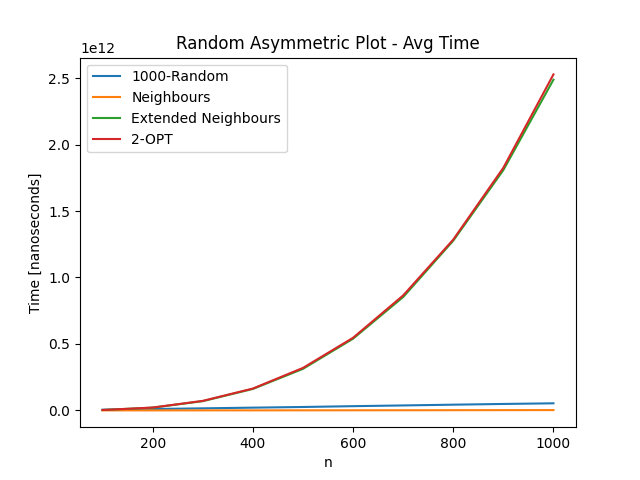
\includegraphics[width=\textwidth, 
                   height = 0.4\textheight, 
                   keepaspectratio]
                  {generated_asym_avg_time} 
\end{center}

\begin{center}
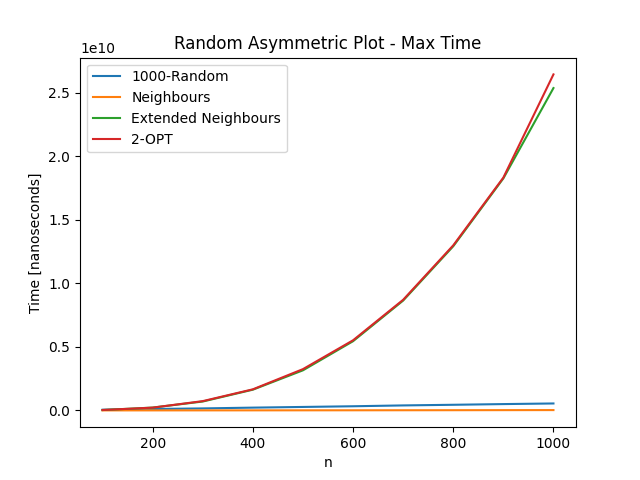
\includegraphics[width=\textwidth, 
                   height = 0.4\textheight, 
                   keepaspectratio]
                  {generated_asym_max_time} 
\end{center}

\subsubsection{Grafy symetryczne}

\begin{center}
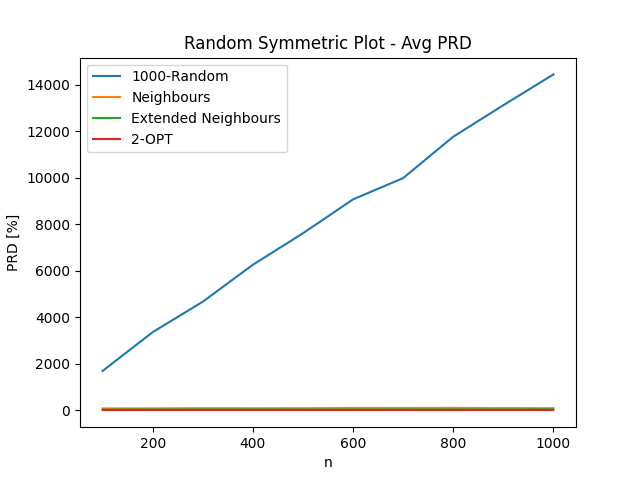
\includegraphics[width=\textwidth, 
                   height = 0.4\textheight, 
                   keepaspectratio]
                  {generated_sym_avg_prd} 
\end{center}

\begin{center}
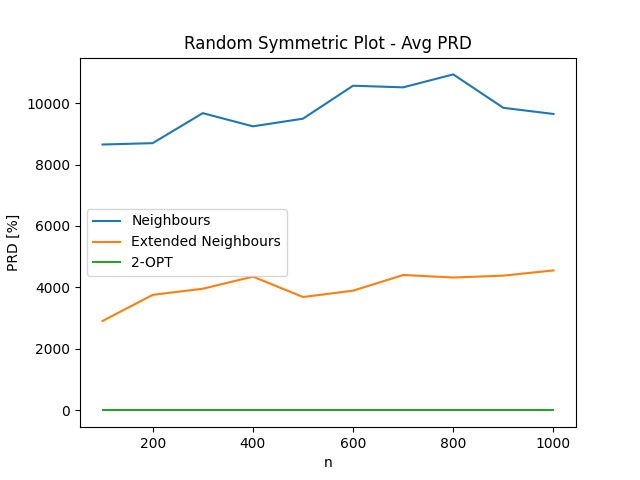
\includegraphics[width=\textwidth, 
                   height = 0.4\textheight, 
                   keepaspectratio]
                  {generated_sym_avg_prd_no_krandom} 
\end{center}

\begin{center}
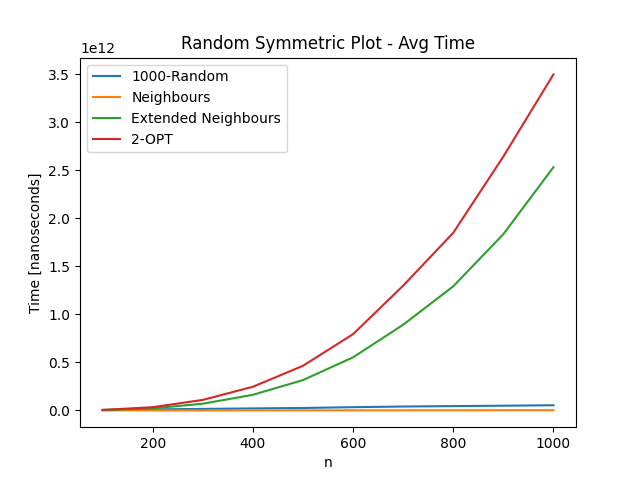
\includegraphics[width=\textwidth, 
                   height = 0.4\textheight, 
                   keepaspectratio]
                  {generated_sym_avg_time} 
\end{center}

\begin{center}
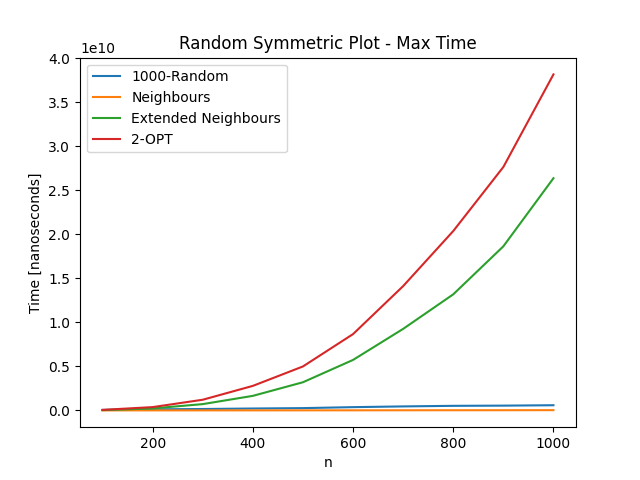
\includegraphics[width=\textwidth, 
                   height = 0.4\textheight, 
                   keepaspectratio]
                  {generated_sym_max_time} 
\end{center}

\subsubsection{Grafy euklidesowe}

\begin{center}
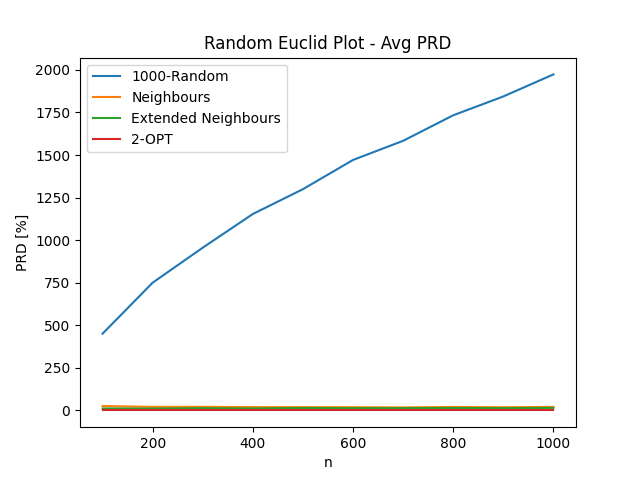
\includegraphics[width=\textwidth, 
                   height = 0.4\textheight, 
                   keepaspectratio]
                  {generated_euclid_avg_prd} 
\end{center}

\begin{center}
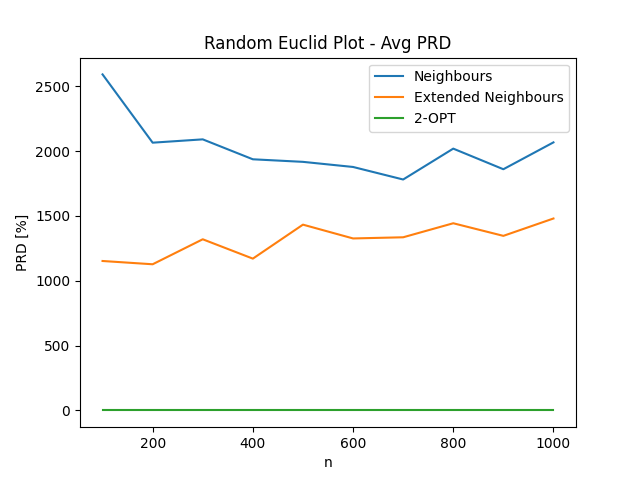
\includegraphics[width=\textwidth, 
                   height = 0.4\textheight, 
                   keepaspectratio]
                  {generated_euclid_avg_prd_no_krandom} 
\end{center}

\begin{center}
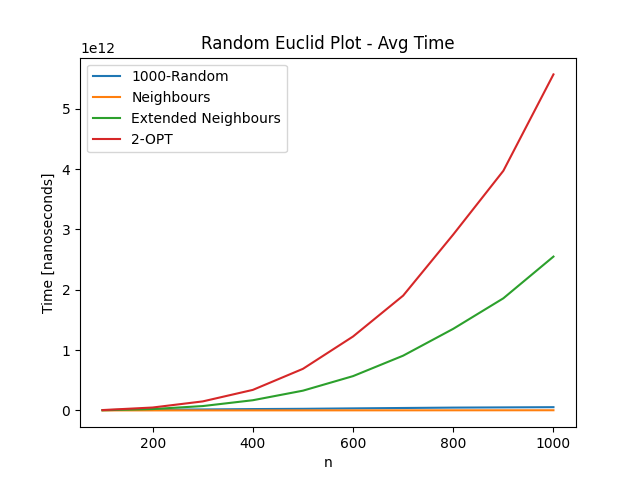
\includegraphics[width=\textwidth, 
                   height = 0.4\textheight, 
                   keepaspectratio]
                  {generated_euclid_avg_time} 
\end{center}

\begin{center}
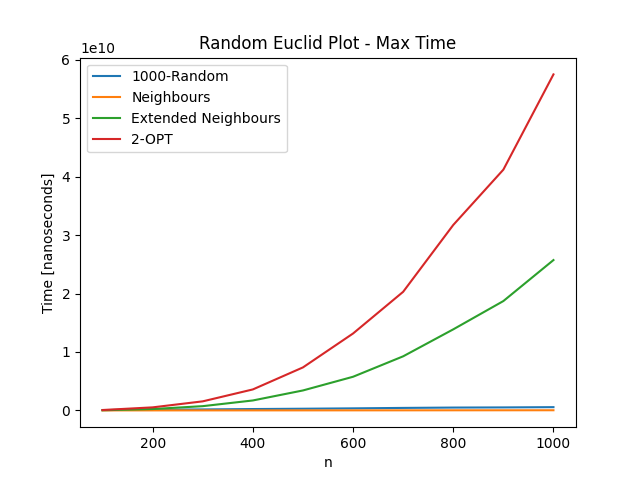
\includegraphics[width=\textwidth, 
                   height = 0.4\textheight, 
                   keepaspectratio]
                  {generated_euclid_max_time} 
\end{center}

\subsection{Wnioski}

W każdej rodzinie grafów najlepsze wyniki (najniższe PRD) miał algorytm 2-OPT z przybliżeniem początkowym Extended Neighbours. Dla grafów asymetrycznych zbliżone wyniki miał sam algorytm Extended Neighbours. Zdecydowanie najgorsze, rosnące liniowo PRD, miał w każdym przypadku algorytm 1000-Random.

Pod względem czasu najlepszy był algorytm Neighbours, który był nieznacznie szybszy od 1000-Random (losowe dane są jak widać generowane powoli). W przypadku rodzin grafów symetrycznych i euklidesowych kolejnym, znacznie wolniejszym algorytmem był algorytm Extended Neighbours (ponieważ wykonuje algorytm Neighbours n razy), a stawkę zamykał korzystający z niego dla początkowego przybliżenia 2-OPT. W przypadku algorytmów asymetrycznych wyniki czasowe dla Extended Neighbours i 2-OPT były bardzo zbliżone.

Algorytm 1000-Random nie jest w żadnym stopniu alternatywą dla innych testowanych algorytmów. Jeśli zależy nam na czasie, powinniśmy użyć delikatnie szybszego, a dającego nieporównywalnie lepsze wyniki algorytmu Neighbours, natomiast jeśli zależy nam na jakości rozwiązania, zdecydowanie najlepszy, choć i najwolniejszy jest algorytm 2-OPT (a dla grafów asymetrycznych również Extended Neighbours).


\section{Porównanie 2-OPT w zależności od przybliżenia początkowego}
\subsection{Tabele}

\subsubsection{Grafy asymetryczne}

\begin{center}
\begin{tabular}{|c|c|c|c|c|c|c|}
\hline
\multicolumn{7}{|c|}{\textbf{Asymmetric Graphs with 2-OPT}}\\
\hline
 & \multicolumn{2}{|c|}{\textbf{AVG Time}} & \multicolumn{2}{|c|}{\textbf{MAX Time}} & \multicolumn{2}{|c|}{\textbf{AVG PRD}}\\
\hline
\textbf{n} & 1000-Random & Ext-Neighbours & 1000-Random & Ext-Neighbours & 1000-Random & Ext-Neighbours\\
\hline
50 & 48453200 & 6136500 & 3738398333 & 489811666 & 355.04376268311 & 0\\
\hline
100 & 140853600 & 35301100 & 11970911666 & 3169770000 & 730.9758129217 & 0\\
\hline
150 & 337295400 & 98910400 & 29113163333 & 9698358333 & 962.98438783734 & 0\\
\hline
200 & 643440000 & 222620100 & 58731895000 & 21984178333 & 1190.65961691776 & 0\\
\hline
250 & 1392918200 & 438522000 & 123776605000 & 43217630000 & 1446.62881606517 & 0\\
\hline
300 & 1981728700 & 744836600 & 181790746666 & 72750526666 & 1684.84457767615 & 0\\
\hline
350 & 3127470800 & 1156490900 & 294949878333 & 114528933333 & 2018.59192018144 & 0\\
\hline
400 & 4895469300 & 1719545200 & 434607098333 & 170149210000 & 2190.69640333427 & 0\\
\hline
450 & 6997186800 & 2429447700 & 638500593333 & 241024308333 & 2315.9713570598 & 0\\
\hline
500 & 10230351100 & 3378707200 & 905001025000 & 331310758333 & 2498.60481496935 & 0\\
\hline
\end{tabular}
\end{center}


\subsubsection{Grafy symetryczne}

\begin{center}
\begin{tabular}{|c|c|c|c|c|c|c|}
\hline
\multicolumn{7}{|c|}{\textbf{Symmetric Graphs with 2-OPT}}\\
\hline
 & \multicolumn{2}{|c|}{\textbf{AVG Time}} & \multicolumn{2}{|c|}{\textbf{MAX Time}} & \multicolumn{2}{|c|}{\textbf{AVG PRD}}\\
\hline
\textbf{n} & 1000-Random & Ext-Neighbours & 1000-Random & Ext-Neighbours & 1000-Random & Ext-Neighbours\\
\hline
50 & 54974700 & 8059300 & 4912670000 & 742475000 & 435.01603975448376 & 0\\
\hline
100 & 263593200 & 79644600 & 24933430000 & 6215445000 & 296.5871346219297 & 76.26814793409217\\
\hline
150 & 854941600 & 252056300 & 79812985000 & 21103678333 & 562.0643403667292 & 0\\
\hline
200 & 1974940700 & 463551300 & 190022033333 & 43272870000 & 386.77781639316737 & 0\\
\hline
250 & 3901226900 & 977426600 & 381697053333 & 91518833333 & 435.57918990772185 & 0\\
\hline
300 & 6813259300 & 1703896100 & 653903618333 & 152749565000 & 527.1451034832014 & 0\\
\hline
350 & 10818486000 & 2609217900 & 1042695165000 & 247398490000 & 371.06322593105233 & 0\\
\hline
400 & 15996929900 & 4046430100 & 1577727018333 & 354304303333 & 351.7245426245308 & 0\\
\hline
450 & 22753961100 & 5739451900 & 2246563521666 & 524977991666 & 510.1009193872297 & 0\\
\hline
500 & 31306288200 & 7293158000 & 3088863130000 & 682899385000 & 423.6764076969968 & 0\\
\hline
\end{tabular}
\end{center}


\subsubsection{Grafy euklidesowe}

\begin{center}
\begin{tabular}{|c|c|c|c|c|c|c|}
\hline
\multicolumn{7}{|c|}{\textbf{Euclid Graphs with 2-OPT}}\\
\hline
 & \multicolumn{2}{|c|}{\textbf{AVG Time}} & \multicolumn{2}{|c|}{\textbf{MAX Time}} & \multicolumn{2}{|c|}{\textbf{AVG PRD}}\\
\hline
\textbf{n} & 1000-Random & Ext-Neighbours & 1000-Random & Ext-Neighbours & 1000-Random & Ext-Neighbours\\
\hline
50 & 50845700 & 7325400 & 4806420000 & 695278000 & 2596.308721025397 & 0\\
\hline
100 & 236384300 & 50275900 & 22503444000 & 4360152000 & 4683.4335972388535 & 0\\
\hline
150 & 748642900 & 159204100 & 71871182000 & 15081932000 & 4791.206250105386 & 0\\
\hline
200 & 1752181800 & 360983300 & 173144656000 & 33194196000 & 5703.476754080477 & 0\\
\hline
250 & 3597519600 & 719419300 & 336032994000 & 66473034000 & 6640.879179142622 & 0\\
\hline
300 & 6177012400 & 1247142900 & 584690090000 & 115264876000 & 8480.93216294145 & 0\\
\hline
350 & 9811912400 & 2034889600 & 950499916000 & 179479596000 & 8406.706667218925 & 0\\
\hline
400 & 14885090600 & 2743647200 & 1429223796000 & 263122394000 & 9456.626662228227 & 0\\
\hline
450 & 20679005000 & 3990645200 & 2027474658000 & 374963440000 & 10298.344279214956 & 0\\
\hline
500 & 30105890700 & 5752855600 & 2857272732000 & 527189884000 & 10733.905445781715 & 0\\
\hline
\end{tabular}
\end{center}



\subsection{Wykresy}

\subsubsection{Grafy asymetryczne}

\begin{center}
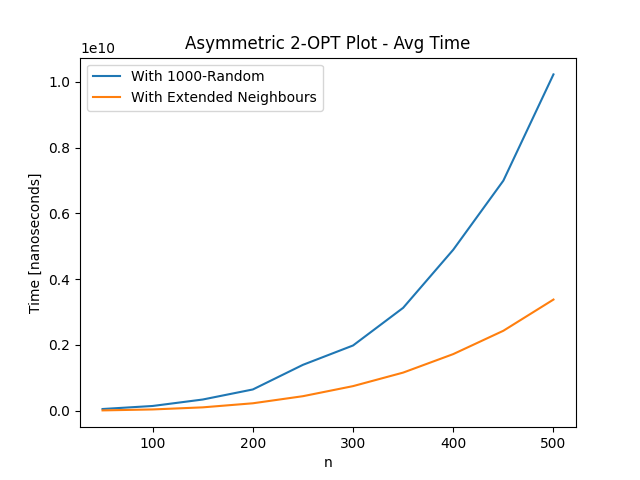
\includegraphics[width=\textwidth, 
                   height = 0.4\textheight, 
                   keepaspectratio]
                  {two_opt_asym_avg_time} 
\end{center}

\begin{center}
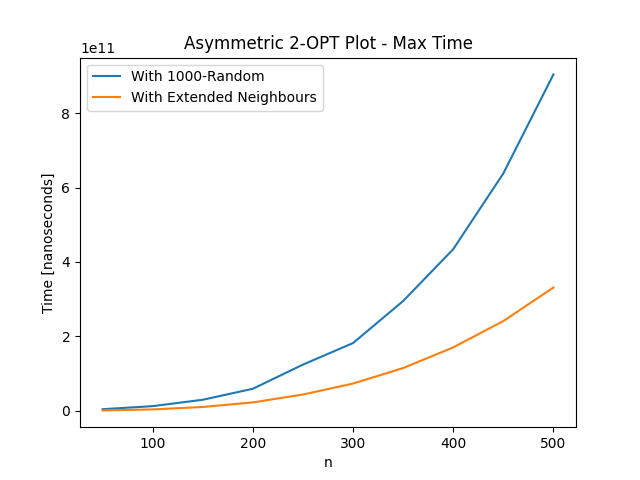
\includegraphics[width=\textwidth, 
                   height = 0.4\textheight, 
                   keepaspectratio]
                  {two_opt_asym_max_time} 
\end{center}

\begin{center}
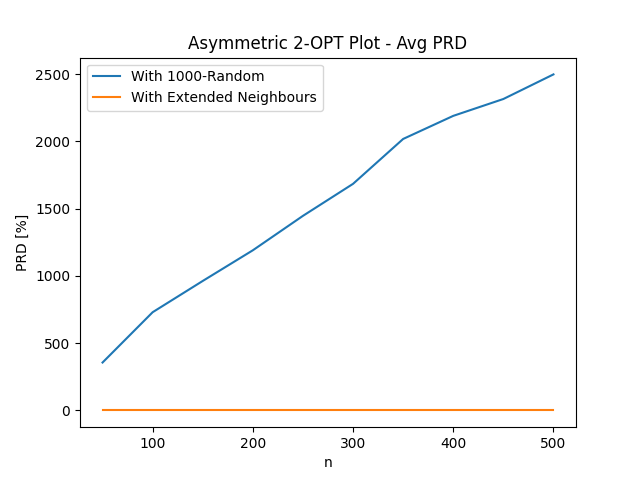
\includegraphics[width=\textwidth, 
                   height = 0.4\textheight, 
                   keepaspectratio]
                  {two_opt_asym_avg_prd} 
\end{center}

\subsubsection{Grafy symetryczne}

\begin{center}
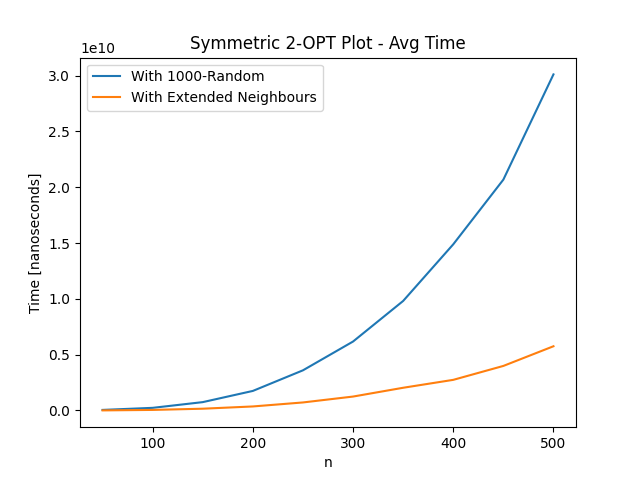
\includegraphics[width=\textwidth, 
                   height = 0.4\textheight, 
                   keepaspectratio]
                  {two_opt_sym_avg_time} 
\end{center}

\begin{center}
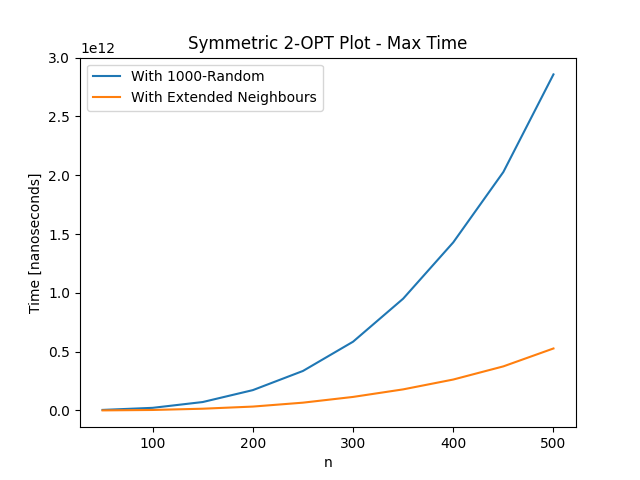
\includegraphics[width=\textwidth, 
                   height = 0.4\textheight, 
                   keepaspectratio]
                  {two_opt_sym_max_time} 
\end{center}

\begin{center}
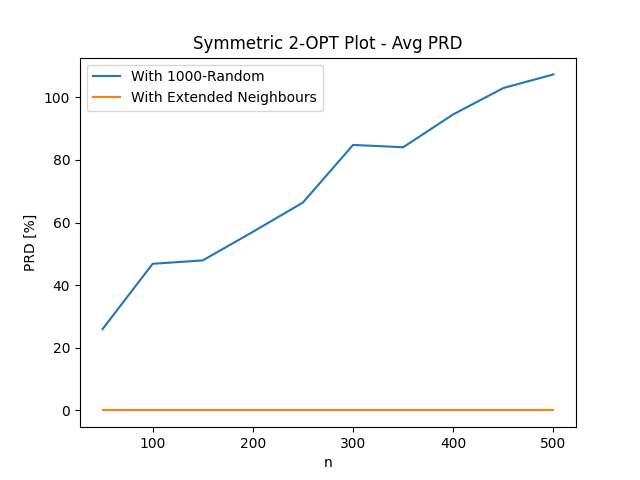
\includegraphics[width=\textwidth, 
                   height = 0.4\textheight, 
                   keepaspectratio]
                  {two_opt_sym_avg_prd} 
\end{center}

\subsubsection{Grafy euklidesowe}

\begin{center}
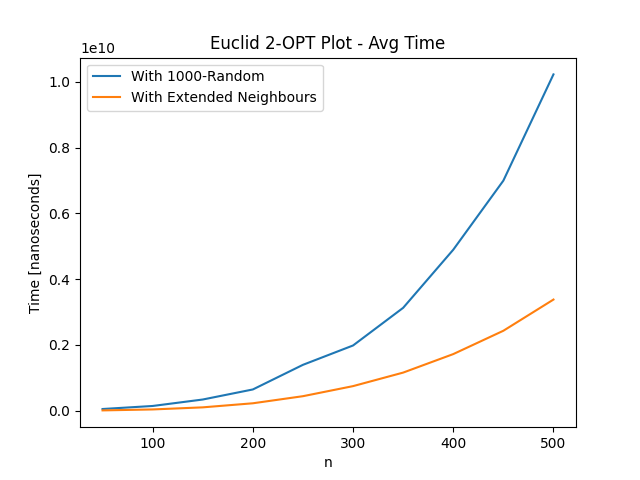
\includegraphics[width=\textwidth, 
                   height = 0.4\textheight, 
                   keepaspectratio]
                  {two_opt_euclid_avg_time} 
\end{center}

\begin{center}
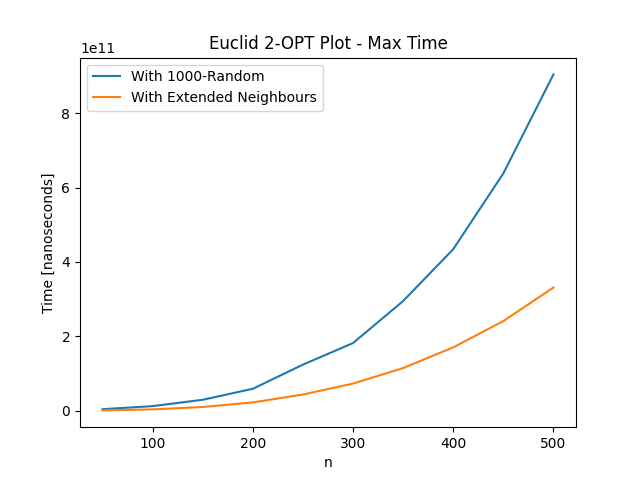
\includegraphics[width=\textwidth, 
                   height = 0.4\textheight, 
                   keepaspectratio]
                  {two_opt_euclid_max_time} 
\end{center}

\begin{center}
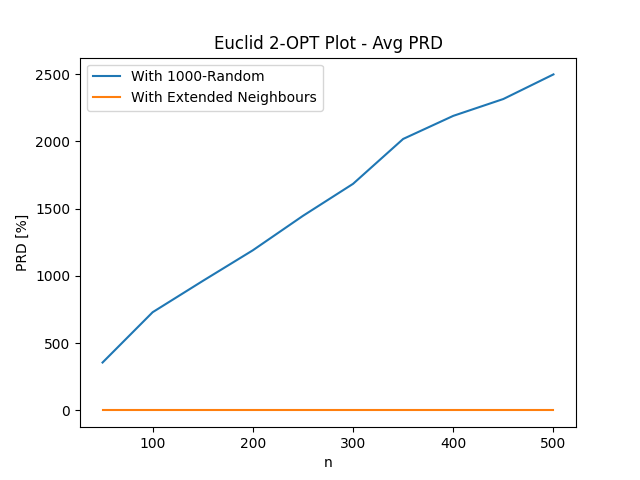
\includegraphics[width=\textwidth, 
                   height = 0.4\textheight, 
                   keepaspectratio]
                  {two_opt_euclid_avg_prd} 
\end{center}
                  
\subsection{Wnioski}

W tym eksperymencie testowany był algorytm 2-OPT z przybliżeniem początkowym na podstawie 1000-Random oraz Extended Neighbours. Pomimo znacznie dłuższego wykonywania się algorytmu Extended Neighbours, co widać w poprzednim eksperymencie, dla każdego typu grafów algorytm korzystający z początkowego przybliżenia 1000-Random był znacznie wolniejszy. Jego PRD natomiast rosło również liniowo w stosunku do lepszego w praktycznie każdym miejscu algorytmu z Extended Neighbours.

Zatem w przypadku 2-OPT bardzo ważne jest początkowe przybliżenie, ponieważ im gorsze początkowe przybliżenie, tym dłużej będzie się wykonywał algorytm oraz tym gorsze wyniki będzie on dawał.

\end{document}